\documentclass[]{article}
\usepackage{lmodern}
\usepackage{amssymb,amsmath}
\usepackage{ifxetex,ifluatex}
\usepackage{fixltx2e} % provides \textsubscript
\ifnum 0\ifxetex 1\fi\ifluatex 1\fi=0 % if pdftex
  \usepackage[T1]{fontenc}
  \usepackage[utf8]{inputenc}
\else % if luatex or xelatex
  \ifxetex
    \usepackage{mathspec}
  \else
    \usepackage{fontspec}
  \fi
  \defaultfontfeatures{Ligatures=TeX,Scale=MatchLowercase}
\fi
% use upquote if available, for straight quotes in verbatim environments
\IfFileExists{upquote.sty}{\usepackage{upquote}}{}
% use microtype if available
\IfFileExists{microtype.sty}{%
\usepackage{microtype}
\UseMicrotypeSet[protrusion]{basicmath} % disable protrusion for tt fonts
}{}
\usepackage[margin=1in]{geometry}
\usepackage{hyperref}
\hypersetup{unicode=true,
            pdftitle={Individual participant data meta-analysis. When? Why? How? A scoping review},
            pdfauthor={Michail Belias},
            pdfborder={0 0 0},
            breaklinks=true}
\urlstyle{same}  % don't use monospace font for urls
\usepackage{longtable,booktabs}
\usepackage{graphicx,grffile}
\makeatletter
\def\maxwidth{\ifdim\Gin@nat@width>\linewidth\linewidth\else\Gin@nat@width\fi}
\def\maxheight{\ifdim\Gin@nat@height>\textheight\textheight\else\Gin@nat@height\fi}
\makeatother
% Scale images if necessary, so that they will not overflow the page
% margins by default, and it is still possible to overwrite the defaults
% using explicit options in \includegraphics[width, height, ...]{}
\setkeys{Gin}{width=\maxwidth,height=\maxheight,keepaspectratio}
\IfFileExists{parskip.sty}{%
\usepackage{parskip}
}{% else
\setlength{\parindent}{0pt}
\setlength{\parskip}{6pt plus 2pt minus 1pt}
}
\setlength{\emergencystretch}{3em}  % prevent overfull lines
\providecommand{\tightlist}{%
  \setlength{\itemsep}{0pt}\setlength{\parskip}{0pt}}
\setcounter{secnumdepth}{0}
% Redefines (sub)paragraphs to behave more like sections
\ifx\paragraph\undefined\else
\let\oldparagraph\paragraph
\renewcommand{\paragraph}[1]{\oldparagraph{#1}\mbox{}}
\fi
\ifx\subparagraph\undefined\else
\let\oldsubparagraph\subparagraph
\renewcommand{\subparagraph}[1]{\oldsubparagraph{#1}\mbox{}}
\fi

%%% Use protect on footnotes to avoid problems with footnotes in titles
\let\rmarkdownfootnote\footnote%
\def\footnote{\protect\rmarkdownfootnote}

%%% Change title format to be more compact
\usepackage{titling}

% Create subtitle command for use in maketitle
\providecommand{\subtitle}[1]{
  \posttitle{
    \begin{center}\large#1\end{center}
    }
}

\setlength{\droptitle}{-2em}

  \title{Individual participant data meta-analysis. When? Why? How? A scoping
review}
    \pretitle{\vspace{\droptitle}\centering\huge}
  \posttitle{\par}
    \author{Michail Belias}
    \preauthor{\centering\large\emph}
  \postauthor{\par}
      \predate{\centering\large\emph}
  \postdate{\par}
    \date{May 13, 2019}

\usepackage{booktabs}
\usepackage{longtable}
\usepackage{array}
\usepackage{multirow}
\usepackage{wrapfig}
\usepackage{float}
\usepackage{colortbl}
\usepackage{pdflscape}
\usepackage{tabu}
\usepackage{threeparttable}
\usepackage{threeparttablex}
\usepackage[normalem]{ulem}
\usepackage{makecell}
\usepackage{xcolor}

\usepackage{booktabs}
\usepackage{longtable}
\usepackage{array}
\usepackage{multirow}
\usepackage{wrapfig}
\usepackage{float}
\usepackage{colortbl}
\usepackage{pdflscape}
\usepackage{tabu}
\usepackage{threeparttable}
\usepackage{threeparttablex}
\usepackage[normalem]{ulem}
\usepackage{makecell}
\usepackage{xcolor}

\begin{document}
\maketitle

\hypertarget{abstract}{%
\section{Abstract}\label{abstract}}

\hypertarget{background}{%
\subsection{Background}\label{background}}

Individual participant data(IPD) meta-analysis(MA) is considered the
gold standard for evidence based inference. It is well established that
IPD-MA offers great advantages compared to aggregate MA and single
studies. Therefore, several systematic reviews have been conducted in
order to investigate current practice and provide guidance. Besides the
characteristics of the meta-analyses (size, design, type of outcome)
most reviews report the primary goal (subgroup analysis, risk factor
assessment) and subsequently the statistical approaches applied.
Nevertheless, last five years no review has been published, while new
guidance is present. Furthermore, past reviews were narrowed down to
specific IPD-MA advantages (For instance subgroup analysis or
modelling).

\textbf{Objective:} Our goal is to conduct a scoping review of IPD-MA
and summarise the aforementioned characteristics. Consequently, we aim
to inform how IPD-MA are performed, what was their goal, which
statistical approach they used and whether all above were clearly
described according to PRISMA guidelines and/or to the level that the
analysis can be reproduced.

\hypertarget{methods}{%
\subsection{Methods}\label{methods}}

We searched MEDLINE and the Cochrane Library \textbf{(we can include
more databases i.e.~EMBASE etc.)} for IPD-MA to identify IPD-MAs
performed the last five years. We excluded diagnostic IPD-MA. We
screened the abstracts and extracted the size of MA, their primary goal,
outcome(s), study designs included, statistical analysis and modelling
approach performed. We report if information was unclear or not reported
and considered the full-text.

\hypertarget{results}{%
\subsection{Results}\label{results}}

Our search resulted in 1538 articles, after exclusion criteria we ended
with \emph{xxx}. We showed an increase per year in IPD-MAs performed.
`The two most predominant medical fields were Cancer \emph{(16\%)},
Cardiovascular diseases \emph{(16\%)} and Mental health \emph{(10\%)}.
An increasing trend in both IPD-MA in general and specifically in
one-stage methods per year has been showed. Nevertheless, more
information should be provided in both the abstract and the article over
the statistical approaches followed.'

\emph{Temporary}

\textbf{Most of the IPD-MAs had as a goal to investigate for subgroups
effects.} \textbf{Reporting type of }

\hypertarget{conclusions}{%
\subsection{Conclusions}\label{conclusions}}

\emph{Not yet}

\newpage

\hypertarget{introduction}{%
\section{Introduction}\label{introduction}}

Meta-analysis (MA) is a statistical method that involves combining
information from multiple sources. While initially, meta-analyses were
limited in aggregated data (AD) in the early 1990s individual
participant data meta-analysis (IPD-MA or IPDMA) was introduced
(CHALMERS 1993). In IPD-MA the participant level information is
available and therefore evidence from multiple studies can be analysed
centrally. Collecting the IPD may be a difficult and time consuming
task, but nevertheless IPD-MA is considered the gold standard in
evidence synthesis (Stewart and Parmar 1993 ; and 1995 ; Stewart and
Tierney 2002) and offers great opportunities (Walraven 2010) that in
AD-MA are considered impossible. Besides when investigating overall
treatment effects where AD-MA and IPD-MA are mathematically equivalent,
IPD-MA offers (1) the possibility to standardize subgroup definitions
and outcomes across studies, (2) higher validity and credibility of
subgroup findings, (3) increased flexibility to search for subgroups
based on combinations of patient and/or disease characteristics (4) the
possibility to avoid ecological BIAS (5) investigate non-linear
functional forms (6) training better prediction models and (7)
efficiently synthesizing evidence from different designs. Given these
advantages systematic reviews were typically applied to inform of how
are IPD from multiple sources analysed and what for. For instance,
Simmonds et al (Simmonds et al. 2005) identified 44 IPD-MAs performed
during 2000-2005 time period and 1) summarized whether IPD-MAs obtained
all the data they sought 2) reported the types of approaches that were
used in the analysis 3) and whether the effects of covariates have been
investigated and 4) report which medical field was their topic. On a
subsequent paper, 10 years later Simmonds et al.~(Simmonds, Stewart, and
Stewart 2015) identified 1371 potential IPD-MAs performed during
2010-2015 time period, sampled 184 of them and after obtaining full
texts included 100 IPD-MAs. Then they investigated along with the topics
investigated in the initial paper they investigated also the quality of
IPD-MA reporting. Riley et al.~(Riley, Lambert, and Abo-Zaid 2010)
identified 383 IPD-MAs performed form instance until 2009 and summarised
only: 1) their medical field topic and 2) whether they assessed risk or
prognostic factors. Finally, Schuit and Ioannidis (Schuit, Li, and
Ioannidis 2018) identified 327 IPD-MAs performed from inception until
2014. Nevertheless, they restricted their interest in subgroup effects
investigation. Our objective is to conduct a systematic review of IPD-MA
from 2015 onwards and and summarise their properties. Furthermore, we
aim to inform when and how IPD-MA are performed, whether state-of the
art methods are used and whether they are clearly described.

Nevertheless far systematic reviews over the IPD-MA practices are
limited until 2014.

\textbf{Reporting} IPD-MA may be conducted in either one stage or two
stages. In one-stage IPD-MA, a statistical model of choice is applied
and IPD from all studies are analysed simultaneously, whilst accounting
for within-studies clustering of the participants. On the other hand, in
two-stage IPD-MA a statistical model of choice is fitted per study.
Subsequently the estimates extracted are pooled using inverse-variance
meta-analytical methods. Both approaches have a variety of parameters
and results that should be reported in the abstract, the methods and the
results section. An extended version of PRISMA for IPD (Stewart et al.
2015) offers guidance on how to report results in IPD-MA. For instance,
in two-stage IPD-MA 1) heterogeneity measures ( \(I^2\) , Cochran's Q
\(\tau^2\)) 2) and their corresponding methods used 3) forest plots (if
applicable) and 4) use of fixed or random effects models and any other
model assumptions should be described in the Methods section.
Furthermore, in't Hout (IntHout et al. 2016) suggested that prediction
intervals of estimates are also a valuable information and should be
included. On the other hand, in one-stage IPD-MA 1) specification of
one-stage models 2) use of fixed-effect, stratified or random-effects in
the terms of the model and 3) how clustering of patients within studies
was accounted for should be reported in the methods section.

\textbf{Effect modification} Simmonds et al.~(Simmonds, Stewart, and
Stewart 2015) showed that IPD-MA are frequently performed in order to
detect treatment effect modification. The approaches that were mostly
used were one aggregated data meta-analysis approach `meta-regression'
and three IPD-MA approaches, per-subgroup meta-analysis, meta-analysis
of interaction terms and one-stage IPD-MA. Guidance on which method to
choose is available. Specifically, Simmonds and Higgins (Simmonds and
Higgins 2007) mathematically proved that, given some unrealistic
assumptions, one-stage IPD-MA is always more powerful than meta-analysis
of interaction terms and meta-regression. Fisher et al.~(Fisher et al.
2011) also critically reviewed all four approaches. They concluded that
one-stage IPD-MA allows for more complex analysis, but is more difficult
to perform than pooling within-trial interaction terms. Furthermore, Hua
et al.~(Hua et al. 2016) noted that these one-stage IPD-MA using
mixed-effects modelling should also centre the effect modifiers to their
mean, in order to separate across and within trial information and
therefore accounting for ecological bias.

\textbf{Modelling functional forms} IPD-MA may be performed in order to
investigate the role of risk-factors in the prevalence of a disease. In
that case observational studies are typically meta-analysed. Thereto,
IPD-MA may involve modelling also non-linear functional forms. Sauerbrei
and Royston (Sauerbrei and Royston 2011) suggested the use of a two
stage approach. As a first stage a fractional polynomial is selected and
pooling their estimates through a point-wise weighted meta-analytical
process. Subsequently they extended these non-linear associations to
include interactions (Royston and Sauerbrei 2013). Furthermore, splines
may also be applied to detect non-linear associations.

\newpage

\hypertarget{methods-1}{%
\section{Methods}\label{methods-1}}

This study is a scoping review of current practices in IPD-MAs . We
report our study according to the Preferred Reporting Items for
Systematic Reviews and Meta-Analyses (PRISMA) guidelines. No formal
protocol exists for this study.

\hypertarget{ipd-ma-search-and-selection-strategy}{%
\subsection{IPD-MA search and selection
strategy}\label{ipd-ma-search-and-selection-strategy}}

We searched in MEDLINE, PubMed, Cochrane library \textbf{(we can place
more)} for IPD-MA conducted between 01/01/2015 and 01/05/2019, see in
\textbf{Supplementary material} for search strategy. We included IPD-MAs
of either RCTs or observational studies, reporting at least one
intervention in human subjects. We excluded IPD-MAs not written in
English. We also excluded diagnostic and prediction IPD-MAs. We removed
duplicate papers and from series we included only the last article. When
unclear we considered full-text assessment. Any disagreement was solved
by a third reviewer. \textbf{if we have to find one it is suggest
though}

\hypertarget{data-extraction-and-statistical-analysis}{%
\subsection{Data extraction and statistical
analysis}\label{data-extraction-and-statistical-analysis}}

For all eligible papers we extracted information that was classified in
three categories: 1) the reporting of the IPD-MA (such as the medical
field, number of included studies and participants, the goal described
in the abstract); 2) the statistical analysis of the IPD-MA (type of
outcome,type of statistical approach,descriptions of methods, and
assessment of heterogeneity); and 3) the reporting of the results
(forest-plots, how many comparisons were performed, proportion of
statistically significant, reporting of subgroup analyses and/or
interaction terms) and 4) when

\newpage

\hypertarget{results-1}{%
\section{Results}\label{results-1}}

We identified 1538 published IPD-MAs. After exclusion of duplicates and
article without Abstracts and

\begin{longtable}[]{@{}lll@{}}
\caption{Individual participant meta-analysis per medical
field}\tabularnewline
\toprule
\begin{minipage}[b]{0.34\columnwidth}\raggedright
General Medical Field\strut
\end{minipage} & \begin{minipage}[b]{0.18\columnwidth}\raggedright
Frequencies\strut
\end{minipage} & \begin{minipage}[b]{0.18\columnwidth}\raggedright
Percentage\strut
\end{minipage}\tabularnewline
\midrule
\endfirsthead
\toprule
\begin{minipage}[b]{0.34\columnwidth}\raggedright
General Medical Field\strut
\end{minipage} & \begin{minipage}[b]{0.18\columnwidth}\raggedright
Frequencies\strut
\end{minipage} & \begin{minipage}[b]{0.18\columnwidth}\raggedright
Percentage\strut
\end{minipage}\tabularnewline
\midrule
\endhead
\begin{minipage}[t]{0.34\columnwidth}\raggedright
Cardiovascular diseases\strut
\end{minipage} & \begin{minipage}[t]{0.18\columnwidth}\raggedright
52\strut
\end{minipage} & \begin{minipage}[t]{0.18\columnwidth}\raggedright
16.4\%\strut
\end{minipage}\tabularnewline
\begin{minipage}[t]{0.34\columnwidth}\raggedright
Neurology\strut
\end{minipage} & \begin{minipage}[t]{0.18\columnwidth}\raggedright
38\strut
\end{minipage} & \begin{minipage}[t]{0.18\columnwidth}\raggedright
11.99\%\strut
\end{minipage}\tabularnewline
\begin{minipage}[t]{0.34\columnwidth}\raggedright
Cancer\strut
\end{minipage} & \begin{minipage}[t]{0.18\columnwidth}\raggedright
37\strut
\end{minipage} & \begin{minipage}[t]{0.18\columnwidth}\raggedright
11.67\%\strut
\end{minipage}\tabularnewline
\begin{minipage}[t]{0.34\columnwidth}\raggedright
Mental health\strut
\end{minipage} & \begin{minipage}[t]{0.18\columnwidth}\raggedright
28\strut
\end{minipage} & \begin{minipage}[t]{0.18\columnwidth}\raggedright
8.83\%\strut
\end{minipage}\tabularnewline
\begin{minipage}[t]{0.34\columnwidth}\raggedright
Statistical\strut
\end{minipage} & \begin{minipage}[t]{0.18\columnwidth}\raggedright
25\strut
\end{minipage} & \begin{minipage}[t]{0.18\columnwidth}\raggedright
7.89\%\strut
\end{minipage}\tabularnewline
\begin{minipage}[t]{0.34\columnwidth}\raggedright
Pregnancy and childbirth\strut
\end{minipage} & \begin{minipage}[t]{0.18\columnwidth}\raggedright
24\strut
\end{minipage} & \begin{minipage}[t]{0.18\columnwidth}\raggedright
7.57\%\strut
\end{minipage}\tabularnewline
\begin{minipage}[t]{0.34\columnwidth}\raggedright
Child health\strut
\end{minipage} & \begin{minipage}[t]{0.18\columnwidth}\raggedright
22\strut
\end{minipage} & \begin{minipage}[t]{0.18\columnwidth}\raggedright
6.94\%\strut
\end{minipage}\tabularnewline
\begin{minipage}[t]{0.34\columnwidth}\raggedright
Endocrine and metabolism\strut
\end{minipage} & \begin{minipage}[t]{0.18\columnwidth}\raggedright
15\strut
\end{minipage} & \begin{minipage}[t]{0.18\columnwidth}\raggedright
4.73\%\strut
\end{minipage}\tabularnewline
\begin{minipage}[t]{0.34\columnwidth}\raggedright
Gastroenterology\strut
\end{minipage} & \begin{minipage}[t]{0.18\columnwidth}\raggedright
12\strut
\end{minipage} & \begin{minipage}[t]{0.18\columnwidth}\raggedright
3.79\%\strut
\end{minipage}\tabularnewline
\begin{minipage}[t]{0.34\columnwidth}\raggedright
Orthopedics\strut
\end{minipage} & \begin{minipage}[t]{0.18\columnwidth}\raggedright
9\strut
\end{minipage} & \begin{minipage}[t]{0.18\columnwidth}\raggedright
2.84\%\strut
\end{minipage}\tabularnewline
\begin{minipage}[t]{0.34\columnwidth}\raggedright
Lungs and airways\strut
\end{minipage} & \begin{minipage}[t]{0.18\columnwidth}\raggedright
7\strut
\end{minipage} & \begin{minipage}[t]{0.18\columnwidth}\raggedright
2.21\%\strut
\end{minipage}\tabularnewline
\begin{minipage}[t]{0.34\columnwidth}\raggedright
Psychology\strut
\end{minipage} & \begin{minipage}[t]{0.18\columnwidth}\raggedright
7\strut
\end{minipage} & \begin{minipage}[t]{0.18\columnwidth}\raggedright
2.21\%\strut
\end{minipage}\tabularnewline
\begin{minipage}[t]{0.34\columnwidth}\raggedright
Generic Care\strut
\end{minipage} & \begin{minipage}[t]{0.18\columnwidth}\raggedright
5\strut
\end{minipage} & \begin{minipage}[t]{0.18\columnwidth}\raggedright
1.58\%\strut
\end{minipage}\tabularnewline
\begin{minipage}[t]{0.34\columnwidth}\raggedright
Geriatrics\strut
\end{minipage} & \begin{minipage}[t]{0.18\columnwidth}\raggedright
5\strut
\end{minipage} & \begin{minipage}[t]{0.18\columnwidth}\raggedright
1.58\%\strut
\end{minipage}\tabularnewline
\begin{minipage}[t]{0.34\columnwidth}\raggedright
Infectious diseases\strut
\end{minipage} & \begin{minipage}[t]{0.18\columnwidth}\raggedright
5\strut
\end{minipage} & \begin{minipage}[t]{0.18\columnwidth}\raggedright
1.58\%\strut
\end{minipage}\tabularnewline
\begin{minipage}[t]{0.34\columnwidth}\raggedright
Pain\strut
\end{minipage} & \begin{minipage}[t]{0.18\columnwidth}\raggedright
5\strut
\end{minipage} & \begin{minipage}[t]{0.18\columnwidth}\raggedright
1.58\%\strut
\end{minipage}\tabularnewline
\begin{minipage}[t]{0.34\columnwidth}\raggedright
Ear, nose and throat\strut
\end{minipage} & \begin{minipage}[t]{0.18\columnwidth}\raggedright
2\strut
\end{minipage} & \begin{minipage}[t]{0.18\columnwidth}\raggedright
0.63\%\strut
\end{minipage}\tabularnewline
\begin{minipage}[t]{0.34\columnwidth}\raggedright
Gynaecology\strut
\end{minipage} & \begin{minipage}[t]{0.18\columnwidth}\raggedright
2\strut
\end{minipage} & \begin{minipage}[t]{0.18\columnwidth}\raggedright
0.63\%\strut
\end{minipage}\tabularnewline
\begin{minipage}[t]{0.34\columnwidth}\raggedright
Nutrition\strut
\end{minipage} & \begin{minipage}[t]{0.18\columnwidth}\raggedright
2\strut
\end{minipage} & \begin{minipage}[t]{0.18\columnwidth}\raggedright
0.63\%\strut
\end{minipage}\tabularnewline
\begin{minipage}[t]{0.34\columnwidth}\raggedright
Other\strut
\end{minipage} & \begin{minipage}[t]{0.18\columnwidth}\raggedright
2\strut
\end{minipage} & \begin{minipage}[t]{0.18\columnwidth}\raggedright
0.63\%\strut
\end{minipage}\tabularnewline
\begin{minipage}[t]{0.34\columnwidth}\raggedright
Renal Disease\strut
\end{minipage} & \begin{minipage}[t]{0.18\columnwidth}\raggedright
2\strut
\end{minipage} & \begin{minipage}[t]{0.18\columnwidth}\raggedright
0.63\%\strut
\end{minipage}\tabularnewline
\begin{minipage}[t]{0.34\columnwidth}\raggedright
Review\strut
\end{minipage} & \begin{minipage}[t]{0.18\columnwidth}\raggedright
2\strut
\end{minipage} & \begin{minipage}[t]{0.18\columnwidth}\raggedright
0.63\%\strut
\end{minipage}\tabularnewline
\begin{minipage}[t]{0.34\columnwidth}\raggedright
Vaccines\strut
\end{minipage} & \begin{minipage}[t]{0.18\columnwidth}\raggedright
2\strut
\end{minipage} & \begin{minipage}[t]{0.18\columnwidth}\raggedright
0.63\%\strut
\end{minipage}\tabularnewline
\begin{minipage}[t]{0.34\columnwidth}\raggedright
Anaesthesiology\strut
\end{minipage} & \begin{minipage}[t]{0.18\columnwidth}\raggedright
1\strut
\end{minipage} & \begin{minipage}[t]{0.18\columnwidth}\raggedright
0.32\%\strut
\end{minipage}\tabularnewline
\begin{minipage}[t]{0.34\columnwidth}\raggedright
Critical care\strut
\end{minipage} & \begin{minipage}[t]{0.18\columnwidth}\raggedright
1\strut
\end{minipage} & \begin{minipage}[t]{0.18\columnwidth}\raggedright
0.32\%\strut
\end{minipage}\tabularnewline
\begin{minipage}[t]{0.34\columnwidth}\raggedright
Ear,throat \& nose\strut
\end{minipage} & \begin{minipage}[t]{0.18\columnwidth}\raggedright
1\strut
\end{minipage} & \begin{minipage}[t]{0.18\columnwidth}\raggedright
0.32\%\strut
\end{minipage}\tabularnewline
\begin{minipage}[t]{0.34\columnwidth}\raggedright
Pharmakokinetics\strut
\end{minipage} & \begin{minipage}[t]{0.18\columnwidth}\raggedright
1\strut
\end{minipage} & \begin{minipage}[t]{0.18\columnwidth}\raggedright
0.32\%\strut
\end{minipage}\tabularnewline
\begin{minipage}[t]{0.34\columnwidth}\raggedright
Renal disease\strut
\end{minipage} & \begin{minipage}[t]{0.18\columnwidth}\raggedright
1\strut
\end{minipage} & \begin{minipage}[t]{0.18\columnwidth}\raggedright
0.32\%\strut
\end{minipage}\tabularnewline
\begin{minipage}[t]{0.34\columnwidth}\raggedright
Stastical\strut
\end{minipage} & \begin{minipage}[t]{0.18\columnwidth}\raggedright
1\strut
\end{minipage} & \begin{minipage}[t]{0.18\columnwidth}\raggedright
0.32\%\strut
\end{minipage}\tabularnewline
\begin{minipage}[t]{0.34\columnwidth}\raggedright
Wound\strut
\end{minipage} & \begin{minipage}[t]{0.18\columnwidth}\raggedright
1\strut
\end{minipage} & \begin{minipage}[t]{0.18\columnwidth}\raggedright
0.32\%\strut
\end{minipage}\tabularnewline
\bottomrule
\end{longtable}

\newpage

\hypertarget{section-2}{%
\subparagraph{}\label{section-2}}

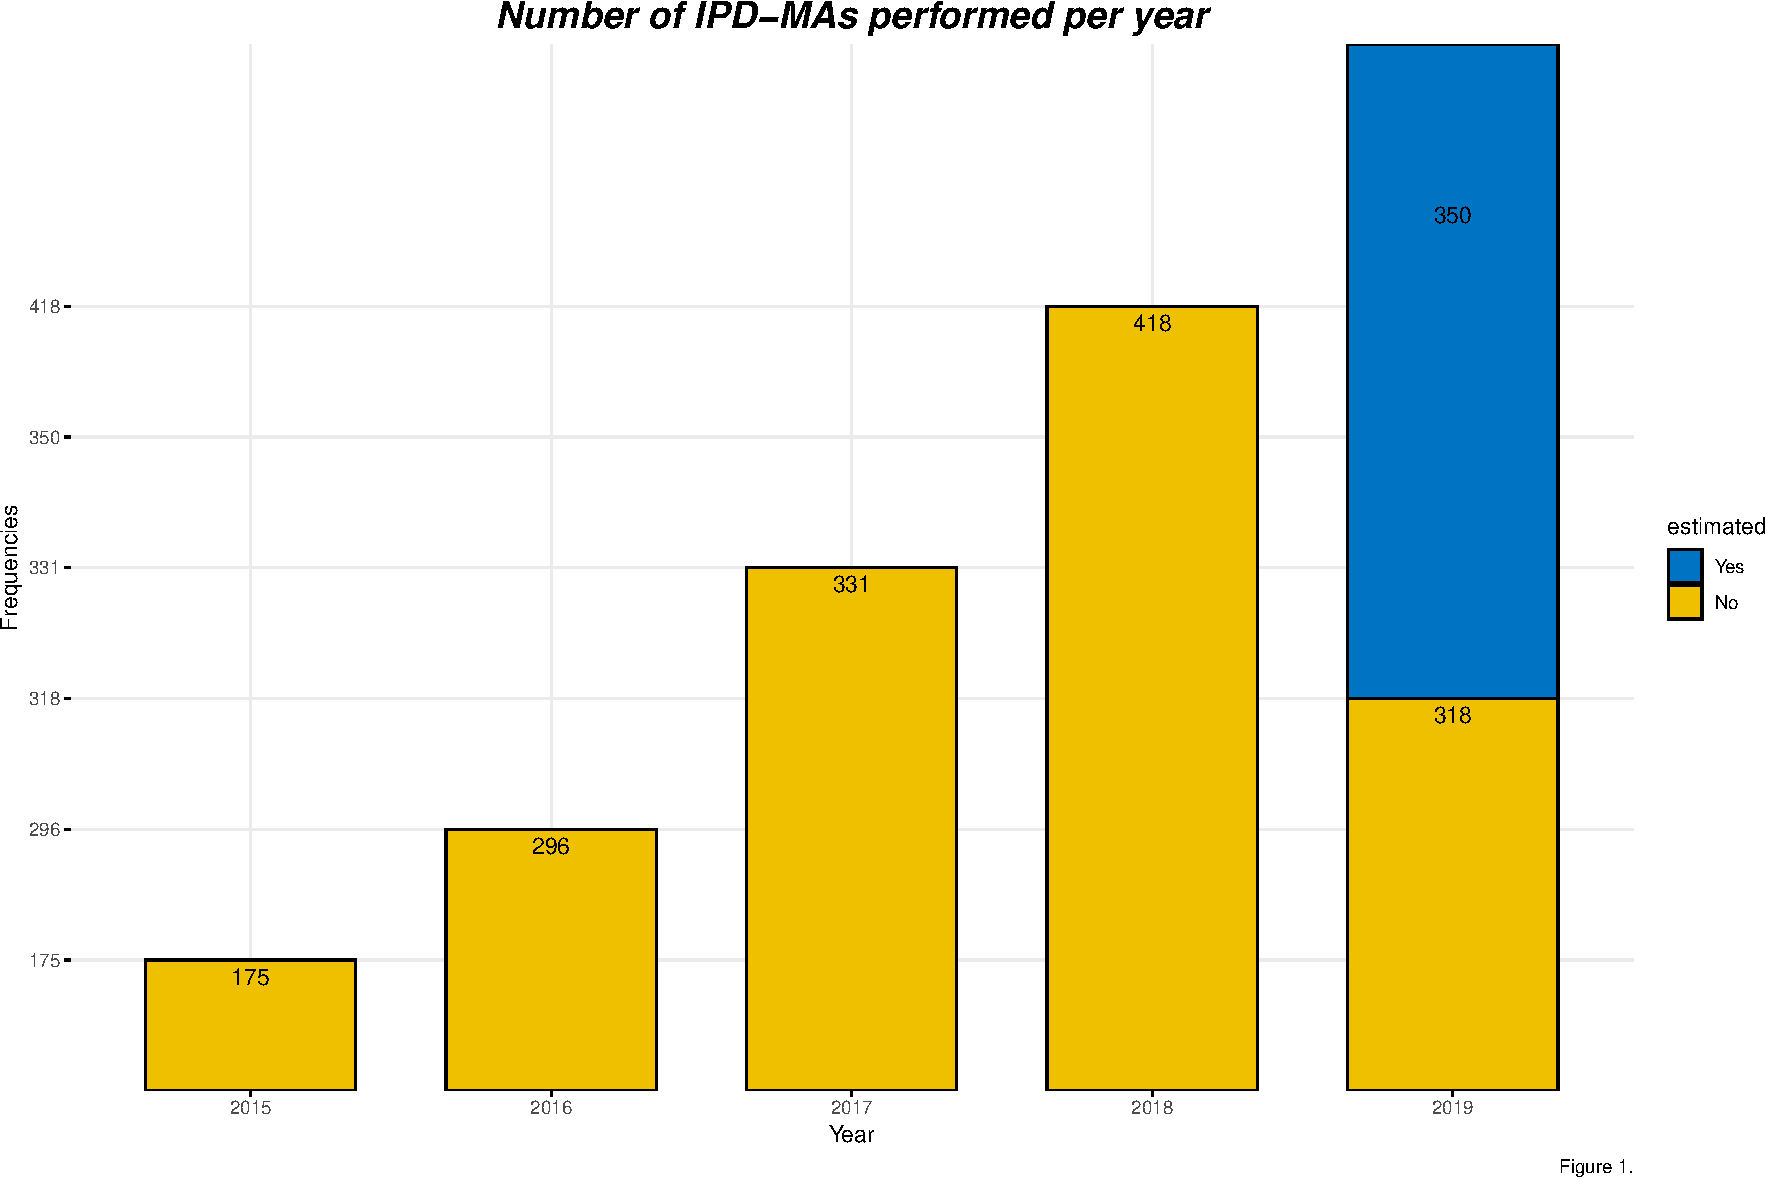
\includegraphics{Figs/unnamed-chunk-3-1.pdf}

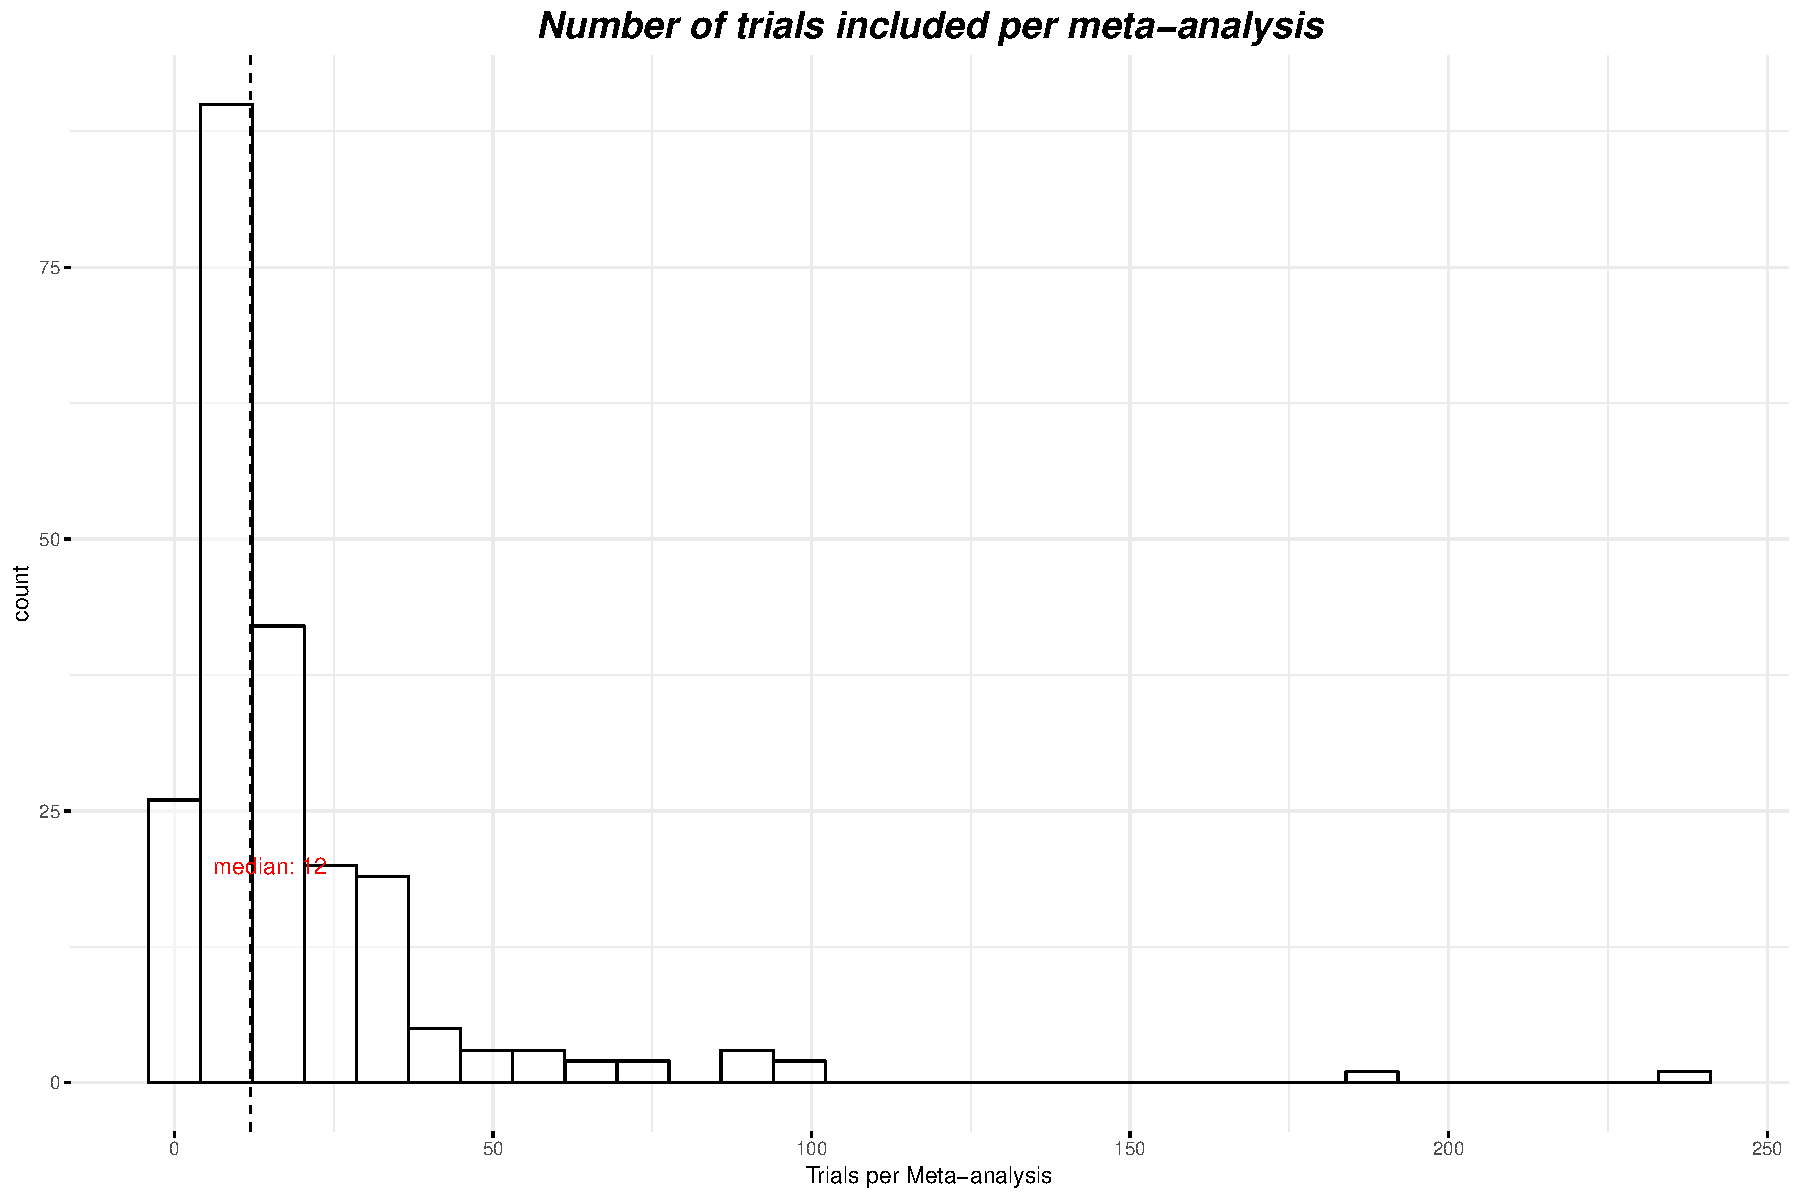
\includegraphics{Figs/unnamed-chunk-4-1.pdf}

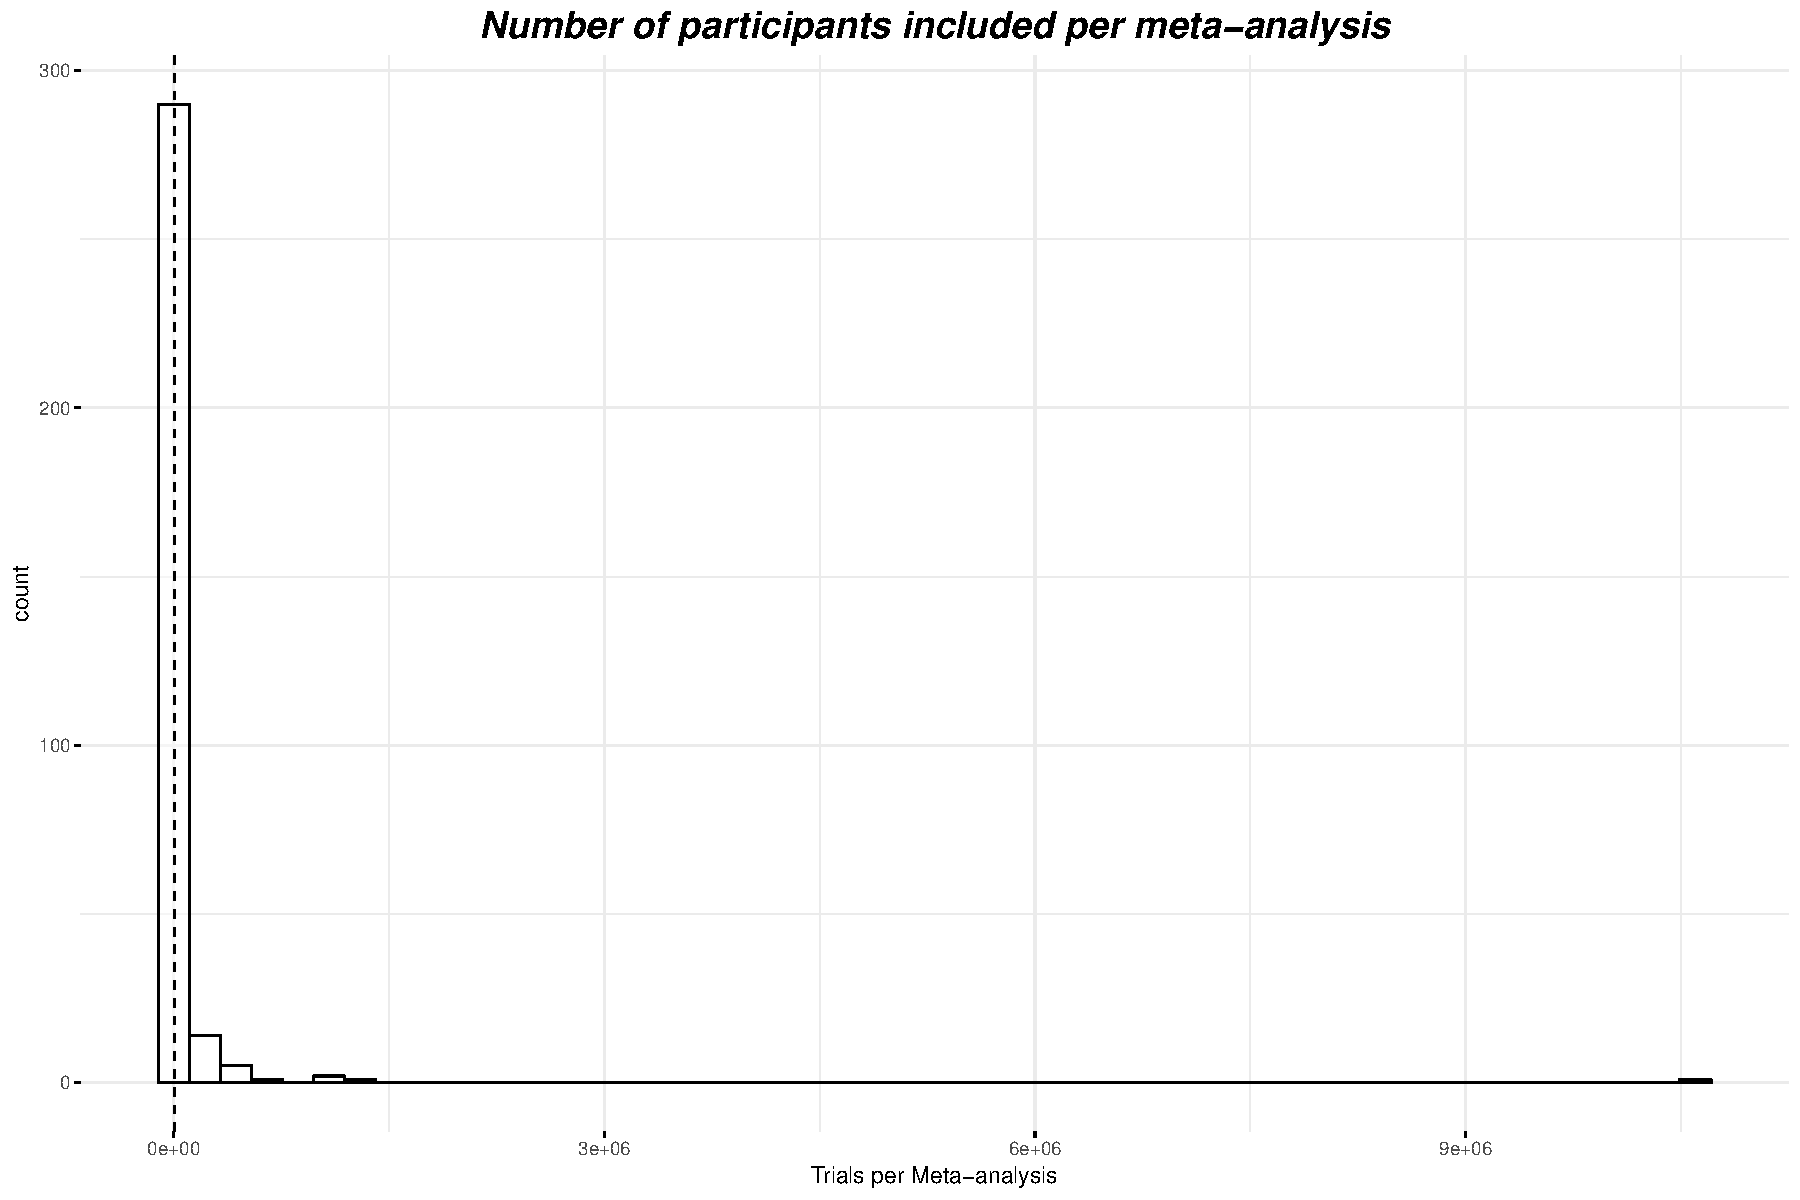
\includegraphics{Figs/unnamed-chunk-5-1.pdf}

\begin{longtable}[]{@{}ll@{}}
\caption{Table 2}\tabularnewline
\toprule
\begin{minipage}[b]{0.34\columnwidth}\raggedright
Type of primary outcome\strut
\end{minipage} & \begin{minipage}[b]{0.18\columnwidth}\raggedright
Frequencies\strut
\end{minipage}\tabularnewline
\midrule
\endfirsthead
\toprule
\begin{minipage}[b]{0.34\columnwidth}\raggedright
Type of primary outcome\strut
\end{minipage} & \begin{minipage}[b]{0.18\columnwidth}\raggedright
Frequencies\strut
\end{minipage}\tabularnewline
\midrule
\endhead
\begin{minipage}[t]{0.34\columnwidth}\raggedright
Binary\strut
\end{minipage} & \begin{minipage}[t]{0.18\columnwidth}\raggedright
11\strut
\end{minipage}\tabularnewline
\begin{minipage}[t]{0.34\columnwidth}\raggedright
Continuous\strut
\end{minipage} & \begin{minipage}[t]{0.18\columnwidth}\raggedright
5\strut
\end{minipage}\tabularnewline
\begin{minipage}[t]{0.34\columnwidth}\raggedright
Time-to-Event\strut
\end{minipage} & \begin{minipage}[t]{0.18\columnwidth}\raggedright
4\strut
\end{minipage}\tabularnewline
\bottomrule
\end{longtable}

\begin{longtable}[]{@{}llllll@{}}
\caption{Table 3}\tabularnewline
\toprule
\begin{minipage}[b]{0.16\columnwidth}\raggedright
\strut
\end{minipage} & \begin{minipage}[b]{0.10\columnwidth}\raggedright
One-stage IPD-MA\strut
\end{minipage} & \begin{minipage}[b]{0.17\columnwidth}\raggedright
Meta-analysis of interaction terms\strut
\end{minipage} & \begin{minipage}[b]{0.16\columnwidth}\raggedright
Per subgroup meta-analysis\strut
\end{minipage} & \begin{minipage}[b]{0.10\columnwidth}\raggedright
Meta-regression\strut
\end{minipage} & \begin{minipage}[b]{0.15\columnwidth}\raggedright
Centered one-stage IPD-MA\strut
\end{minipage}\tabularnewline
\midrule
\endfirsthead
\toprule
\begin{minipage}[b]{0.16\columnwidth}\raggedright
\strut
\end{minipage} & \begin{minipage}[b]{0.10\columnwidth}\raggedright
One-stage IPD-MA\strut
\end{minipage} & \begin{minipage}[b]{0.17\columnwidth}\raggedright
Meta-analysis of interaction terms\strut
\end{minipage} & \begin{minipage}[b]{0.16\columnwidth}\raggedright
Per subgroup meta-analysis\strut
\end{minipage} & \begin{minipage}[b]{0.10\columnwidth}\raggedright
Meta-regression\strut
\end{minipage} & \begin{minipage}[b]{0.15\columnwidth}\raggedright
Centered one-stage IPD-MA\strut
\end{minipage}\tabularnewline
\midrule
\endhead
\begin{minipage}[t]{0.16\columnwidth}\raggedright
\strut
\end{minipage} & \begin{minipage}[t]{0.10\columnwidth}\raggedright
\strut
\end{minipage} & \begin{minipage}[t]{0.17\columnwidth}\raggedright
Fixed vs\strut
\end{minipage} & \begin{minipage}[t]{0.16\columnwidth}\raggedright
random effects\strut
\end{minipage} & \begin{minipage}[t]{0.10\columnwidth}\raggedright
\strut
\end{minipage} & \begin{minipage}[t]{0.15\columnwidth}\raggedright
\strut
\end{minipage}\tabularnewline
\begin{minipage}[t]{0.16\columnwidth}\raggedright
Fixed effect\strut
\end{minipage} & \begin{minipage}[t]{0.10\columnwidth}\raggedright
x\strut
\end{minipage} & \begin{minipage}[t]{0.17\columnwidth}\raggedright
x\strut
\end{minipage} & \begin{minipage}[t]{0.16\columnwidth}\raggedright
x\strut
\end{minipage} & \begin{minipage}[t]{0.10\columnwidth}\raggedright
x\strut
\end{minipage} & \begin{minipage}[t]{0.15\columnwidth}\raggedright
x\strut
\end{minipage}\tabularnewline
\begin{minipage}[t]{0.16\columnwidth}\raggedright
Random effects\strut
\end{minipage} & \begin{minipage}[t]{0.10\columnwidth}\raggedright
x\strut
\end{minipage} & \begin{minipage}[t]{0.17\columnwidth}\raggedright
x\strut
\end{minipage} & \begin{minipage}[t]{0.16\columnwidth}\raggedright
x\strut
\end{minipage} & \begin{minipage}[t]{0.10\columnwidth}\raggedright
x\strut
\end{minipage} & \begin{minipage}[t]{0.15\columnwidth}\raggedright
x\strut
\end{minipage}\tabularnewline
\begin{minipage}[t]{0.16\columnwidth}\raggedright
\strut
\end{minipage} & \begin{minipage}[t]{0.10\columnwidth}\raggedright
\strut
\end{minipage} & \begin{minipage}[t]{0.17\columnwidth}\raggedright
Reporting of\strut
\end{minipage} & \begin{minipage}[t]{0.16\columnwidth}\raggedright
heterogeneity\strut
\end{minipage} & \begin{minipage}[t]{0.10\columnwidth}\raggedright
\strut
\end{minipage} & \begin{minipage}[t]{0.15\columnwidth}\raggedright
\strut
\end{minipage}\tabularnewline
\begin{minipage}[t]{0.16\columnwidth}\raggedright
\(I^2\)\strut
\end{minipage} & \begin{minipage}[t]{0.10\columnwidth}\raggedright
x\strut
\end{minipage} & \begin{minipage}[t]{0.17\columnwidth}\raggedright
x\strut
\end{minipage} & \begin{minipage}[t]{0.16\columnwidth}\raggedright
x\strut
\end{minipage} & \begin{minipage}[t]{0.10\columnwidth}\raggedright
x\strut
\end{minipage} & \begin{minipage}[t]{0.15\columnwidth}\raggedright
x\strut
\end{minipage}\tabularnewline
\begin{minipage}[t]{0.16\columnwidth}\raggedright
Cochran's Q (without \(I^2\))\strut
\end{minipage} & \begin{minipage}[t]{0.10\columnwidth}\raggedright
x\strut
\end{minipage} & \begin{minipage}[t]{0.17\columnwidth}\raggedright
x\strut
\end{minipage} & \begin{minipage}[t]{0.16\columnwidth}\raggedright
x\strut
\end{minipage} & \begin{minipage}[t]{0.10\columnwidth}\raggedright
x\strut
\end{minipage} & \begin{minipage}[t]{0.15\columnwidth}\raggedright
x\strut
\end{minipage}\tabularnewline
\begin{minipage}[t]{0.16\columnwidth}\raggedright
\(\tau^2\)\strut
\end{minipage} & \begin{minipage}[t]{0.10\columnwidth}\raggedright
x\strut
\end{minipage} & \begin{minipage}[t]{0.17\columnwidth}\raggedright
x\strut
\end{minipage} & \begin{minipage}[t]{0.16\columnwidth}\raggedright
x\strut
\end{minipage} & \begin{minipage}[t]{0.10\columnwidth}\raggedright
x\strut
\end{minipage} & \begin{minipage}[t]{0.15\columnwidth}\raggedright
x\strut
\end{minipage}\tabularnewline
\begin{minipage}[t]{0.16\columnwidth}\raggedright
Prediction intervals\strut
\end{minipage} & \begin{minipage}[t]{0.10\columnwidth}\raggedright
x\strut
\end{minipage} & \begin{minipage}[t]{0.17\columnwidth}\raggedright
x\strut
\end{minipage} & \begin{minipage}[t]{0.16\columnwidth}\raggedright
x\strut
\end{minipage} & \begin{minipage}[t]{0.10\columnwidth}\raggedright
x\strut
\end{minipage} & \begin{minipage}[t]{0.15\columnwidth}\raggedright
x\strut
\end{minipage}\tabularnewline
\begin{minipage}[t]{0.16\columnwidth}\raggedright
From one-stage model\strut
\end{minipage} & \begin{minipage}[t]{0.10\columnwidth}\raggedright
x\strut
\end{minipage} & \begin{minipage}[t]{0.17\columnwidth}\raggedright
x\strut
\end{minipage} & \begin{minipage}[t]{0.16\columnwidth}\raggedright
x\strut
\end{minipage} & \begin{minipage}[t]{0.10\columnwidth}\raggedright
x\strut
\end{minipage} & \begin{minipage}[t]{0.15\columnwidth}\raggedright
x\strut
\end{minipage}\tabularnewline
\begin{minipage}[t]{0.16\columnwidth}\raggedright
Other\strut
\end{minipage} & \begin{minipage}[t]{0.10\columnwidth}\raggedright
x\strut
\end{minipage} & \begin{minipage}[t]{0.17\columnwidth}\raggedright
x\strut
\end{minipage} & \begin{minipage}[t]{0.16\columnwidth}\raggedright
x\strut
\end{minipage} & \begin{minipage}[t]{0.10\columnwidth}\raggedright
x\strut
\end{minipage} & \begin{minipage}[t]{0.15\columnwidth}\raggedright
x\strut
\end{minipage}\tabularnewline
\begin{minipage}[t]{0.16\columnwidth}\raggedright
Not reported\strut
\end{minipage} & \begin{minipage}[t]{0.10\columnwidth}\raggedright
x\strut
\end{minipage} & \begin{minipage}[t]{0.17\columnwidth}\raggedright
x\strut
\end{minipage} & \begin{minipage}[t]{0.16\columnwidth}\raggedright
x\strut
\end{minipage} & \begin{minipage}[t]{0.10\columnwidth}\raggedright
x\strut
\end{minipage} & \begin{minipage}[t]{0.15\columnwidth}\raggedright
x\strut
\end{minipage}\tabularnewline
\bottomrule
\end{longtable}

\newpage

\hypertarget{references}{%
\section*{References}\label{references}}
\addcontentsline{toc}{section}{References}

\hypertarget{refs}{}
\leavevmode\hypertarget{ref-Stewart_1995}{}%
and, Lesley A. Stewart. 1995. ``Practical Methodology of Meta-Analyses
(Overviews) Using Updated Individual Patient Data.'' \emph{Statistics in
Medicine} 14 (19): 2057--79.
\url{https://doi.org/10.1002/sim.4780141902}.

\leavevmode\hypertarget{ref-CHALMERS_1993}{}%
CHALMERS, IAIN. 1993. ``The Cochrane Collaboration: Preparing,
Maintaining, and Disseminating Systematic Reviews of the Effects of
Health Care.'' \emph{Annals of the New York Academy of Sciences} 703 (1
Doing More Go): 156--65.
\url{https://doi.org/10.1111/j.1749-6632.1993.tb26345.x}.

\leavevmode\hypertarget{ref-Fisher_2011}{}%
Fisher, D.J., A.J. Copas, J.F. Tierney, and M.K.B. Parmar. 2011. ``A
Critical Review of Methods for the Assessment of Patient-Level
Interactions in Individual Participant Data Meta-Analysis of Randomized
Trials, and Guidance for Practitioners.'' \emph{Journal of Clinical
Epidemiology} 64 (9): 949--67.
\url{https://doi.org/10.1016/j.jclinepi.2010.11.016}.

\leavevmode\hypertarget{ref-Hua_2016}{}%
Hua, Hairui, Danielle L. Burke, Michael J. Crowther, Joie Ensor, Catrin
Tudur Smith, and Richard D. Riley. 2016. ``One-Stage Individual
Participant Data Meta-Analysis Models: Estimation of Treatment-Covariate
Interactions Must Avoid Ecological Bias by Separating Out Within-Trial
and Across-Trial Information.'' \emph{Statistics in Medicine} 36 (5):
772--89. \url{https://doi.org/10.1002/sim.7171}.

\leavevmode\hypertarget{ref-IntHout_2016}{}%
IntHout, Joanna, John P A Ioannidis, Maroeska M Rovers, and Jelle J
Goeman. 2016. ``Plea for Routinely Presenting Prediction Intervals in
Meta-Analysis.'' \emph{BMJ Open} 6 (7): e010247.
\url{https://doi.org/10.1136/bmjopen-2015-010247}.

\leavevmode\hypertarget{ref-Riley_2010}{}%
Riley, R. D., P. C. Lambert, and G. Abo-Zaid. 2010. ``Meta-Analysis of
Individual Participant Data: Rationale, Conduct, and Reporting.''
\emph{BMJ} 340 (feb05 1): c221--c221.
\url{https://doi.org/10.1136/bmj.c221}.

\leavevmode\hypertarget{ref-royston_interaction_2013}{}%
Royston, Patrick, and Willi Sauerbrei. 2013. ``Interaction of Treatment
with a Continuous Variable: Simulation Study of Significance Level for
Several Methods of Analysis.'' \emph{Statistics in Medicine} 32 (22):
3788--3803. \url{https://doi.org/10.1002/sim.5813}.

\leavevmode\hypertarget{ref-Sauerbrei_2011}{}%
Sauerbrei, Willi, and Patrick Royston. 2011. ``A New Strategy for
Meta-Analysis of Continuous Covariates in Observational Studies.''
\emph{Statistics in Medicine} 30 (28): 3341--60.
\url{https://doi.org/10.1002/sim.4333}.

\leavevmode\hypertarget{ref-Schuit_2018}{}%
Schuit, Ewoud, Alvin H Li, and John P A Ioannidis. 2018. ``How Often Can
Meta-Analyses of Individual-Level Data Individualize Treatment? A
Meta-Epidemiologic Study.'' \emph{International Journal of Epidemiology}
48 (2): 596--608. \url{https://doi.org/10.1093/ije/dyy239}.

\leavevmode\hypertarget{ref-Simmonds_2005}{}%
Simmonds, Mark C, Julian P T Higginsa, Lesley A Stewartb, Jayne F
Tierneyb, Mike J Clarke, and Simon G Thompson. 2005. ``Meta-Analysis of
Individual Patient Data from Randomized Trials: A Review of Methods Used
in Practice.'' \emph{Clinical Trials: Journal of the Society for
Clinical Trials} 2 (3): 209--17.
\url{https://doi.org/10.1191/1740774505cn087oa}.

\leavevmode\hypertarget{ref-Simmonds_2015}{}%
Simmonds, Mark, Gavin Stewart, and Lesley Stewart. 2015. ``A Decade of
Individual Participant Data Meta-Analyses: A Review of Current
Practice.'' \emph{Contemporary Clinical Trials} 45 (November): 76--83.
\url{https://doi.org/10.1016/j.cct.2015.06.012}.

\leavevmode\hypertarget{ref-Simmonds_2007}{}%
Simmonds, M. C., and J. P. T. Higgins. 2007. ``Covariate Heterogeneity
in Meta-Analysis: Criteria for Deciding Between Meta-Regression and
Individual Patient Data.'' \emph{Statistics in Medicine} 26 (15):
2982--99. \url{https://doi.org/10.1002/sim.2768}.

\leavevmode\hypertarget{ref-Stewart_1993}{}%
Stewart, L.A, and M.K.B Parmar. 1993. ``Meta-Analysis of the Literature
or of Individual Patient Data: Is There a Difference?'' \emph{The
Lancet} 341 (8842): 418--22.
\url{https://doi.org/10.1016/0140-6736(93)93004-k}.

\leavevmode\hypertarget{ref-Stewart_2015}{}%
Stewart, Lesley A., Mike Clarke, Maroeska Rovers, Richard D. Riley, Mark
Simmonds, Gavin Stewart, and Jayne F. Tierney. 2015. ``Preferred
Reporting Items for a Systematic Review and Meta-Analysis of Individual
Participant Data.'' \emph{JAMA} 313 (16): 1657.
\url{https://doi.org/10.1001/jama.2015.3656}.

\leavevmode\hypertarget{ref-Stewart_2002}{}%
Stewart, Lesley A., and Jayne F. Tierney. 2002. ``To IPD or Not to
IPD?'' \emph{Evaluation \& the Health Professions} 25 (1): 76--97.
\url{https://doi.org/10.1177/0163278702025001006}.

\leavevmode\hypertarget{ref-van_Walraven_2010}{}%
Walraven, Carl van. 2010. ``Individual Patient Meta-Analysisrewards and
Challenges.'' \emph{Journal of Clinical Epidemiology} 63 (3): 235--37.
\url{https://doi.org/10.1016/j.jclinepi.2009.04.001}.


\end{document}
